\documentclass{beamer}

\usepackage[utf8]{inputenc}
\usepackage{pgfpages}
\usepackage{stmaryrd}
\usepackage{amsmath}
\usepackage{listings}
\usepackage{graphicx}

\hypersetup{pdfstartview={Fit}}

\setbeamertemplate{navigation symbols}{}
\setbeamertemplate{footline}
  {\hfill {\normalsize \insertframenumber{}/\inserttotalframenumber{}}}

  
\newcommand{\hastype}{\mathop{:}}

\newcommand{\dand}{\mathbin{\overline{\land}}}
\newcommand{\dnot}{\mathop{\overline{\lnot}}}
\newcommand{\dimpl}{\mathbin{\overline{\to}}}
\newcommand{\dexists}{\mathop{\overline{\exists}}}
\newcommand{\dforall}{\mathop{\overline{\forall}}}

\newcommand{\hsbind}{\mathbin{\texttt{>>=}}}
\newcommand{\hsrevbind}{\mathbin{\texttt{=<<}}}
\newcommand{\hsseq}{\mathbin{\texttt{>>}}}
\newcommand{\occons}{\mathbin{::}}

\newcommand{\statecps}[3]{\llbracket #3 \rrbracket^{#2}_{#1}}
\newcommand{\cps}[2]{\llbracket #2 \rrbracket^{#1}}

\newcommand{\sem}[1]{\llbracket #1 \rrbracket}
\newcommand{\intens}[1]{\overline{#1}}

\newcommand{\obj}[1]{\text{Obj}(#1)}
\newcommand{\inl}[1]{\text{inl}(#1)}
\newcommand{\inr}[1]{\text{inr}(#1)}
\newcommand{\id}[1]{\text{id}_{#1}}



\begin{document}

\title[Effects \& Semantics]{Effects in Natural Language Semantics}
\author{Jiří Maršík}
\institute[INRIA Loria]
{
  Sémagramme \\
  INRIA Loria
}
\date[February 2014]{February 18, 2014}

\frame{\titlepage \setcounter{framenumber}{1}}

\begin{frame}
  \frametitle{A Fistful of Types}

  $\sem{read}$ has had many semantic types

  \vfill

  \begin{tabular}{rl}
    Naive & $\iota \to \iota \to o$ \\
    Type-raised & $((\iota \to o) \to o) \to ((\iota \to o) \to o) \to o$ \\
    Dynamic$_1$ & $((\iota \to \gamma \to (\gamma \to o) \to o) \to \gamma \to (\gamma \to o) \to o)$ \\ & $\to ((\iota \to \gamma \to (\gamma \to o) \to o) \to \gamma \to (\gamma \to o) \to o)$ \\ & $\to \gamma \to (\gamma \to o) \to o$ \\
    Dynamic$_2$ & $(((\gamma \to \iota) \to \gamma \to (\gamma \to o) \to o) \to \gamma \to (\gamma \to o) \to o)$ \\ & $\to (((\gamma \to \iota) \to \gamma \to (\gamma \to o) \to o) \to \gamma \to (\gamma \to o) \to o)$ \\ & $\to \gamma \to (\gamma \to o) \to o$ \\
    Intensional$_1$ & $\iota \to \iota \to \sigma \to o$ \\
    Intensional$_2$ & $(\sigma \to \iota) \to (\sigma \to \iota) \to \sigma \to o$ \\
    Optional & $(\iota \oplus *) \to \iota \to o$ \\
    Events & $\iota \to \iota \to \beta \to \gamma \to (\gamma \to o) \to o$
  \end{tabular}
\end{frame}

\begin{frame}
  \frametitle{For a Few Types More}
  
  \begin{align*}
    \sem{read} & \hastype \, ((((\sigma \to \gamma \to \iota) \to \sigma \to \gamma \to (\gamma \to o) \to o) \\
    & \to \sigma \to \gamma \to (\gamma \to o) \to o) \oplus *) \\
    & \to (((\sigma \to \gamma \to \iota) \to \sigma \to \gamma \to (\gamma \to o) \to o) \\
    & \to \sigma \to \gamma \to (\gamma \to o) \to o) \\
    & \to \beta \to \sigma \to \gamma \to (\gamma \to o) \to o \\
    \sem{read} & \hastype Dyn(Int(Evt(Opt(\iota \to \iota \to o)))) \\
    \sem{read} & =\, ??? \\
  \end{align*}
\end{frame}

\begin{frame}
  \frametitle{Denotational Semantics}

  $p : \alpha \to \beta$

  $p$ an expression of type $\beta$ parametrized by $\alpha$

  \vfill

  $\sem{\alpha}$, $\sem{\beta}$ sets

  \vfill

  $\sem{p} =\; ?$
  \begin{itemize}
  \pause
  \item $\sem{p} : \sem{\alpha} \to \sem{\beta}$ \\
    Total functions, very rare
  \pause
  \item $\sem{p} : \sem{\alpha} \to \sem{\beta}_\bot$ \\
    Partial functions, accounts for divergence and failure
  \pause
  \item $\sem{p} : \sem{\alpha} \to \sem{\beta} \oplus E$ \\
    Exceptions, accounts for handling of exceptions
  \pause
  \item $\sem{p} : \sem{\alpha} \to (\sem{\beta} \times S)^S$ \\
    State, accounts for accessing and modifying variables
  \end{itemize}
\end{frame}

\begin{frame}
  \frametitle{Kleisli triples}

  A \textbf{Kleisli triple} over a category $\mathcal{C}$ is a triple $(T, \eta,
  \_^{*})$, where $T : \obj{\mathcal{C}} \to \obj{\mathcal{C}}$, $\eta_A : A
  \to T A$ for $A \in \obj{\mathcal{C}}$, $f^* : T A \to T B$ for $f : A \to T
  B$ and the following equations hold:

  \begin{itemize}
  \item $\eta_A^* = \id{T A}$
  \item $\eta_A; f^* = f$ for $f : A \to T B$
  \item $f^*; g^* = (f;g^*)^*$ for $f : A \to T B$ and $g : B \to T C$.
  \end{itemize}

  \pause

  \begin{block}{Kleisli category}
    \begin{itemize}
    \item $\obj{\mathcal{C}_T} = \obj{\mathcal{C}}$
    \item $\mathcal{C}_T(A, B) = \mathcal{C}(A, T B)$
    \item the identity on A in $\mathcal{C}_T$ is $\eta_A : A \to T A$
    \item the composition of $f$ and $g$ is $f; g^*$
    \end{itemize}
  \end{block}
\end{frame}

\begin{frame}
  \frametitle{Examples of Kleisli triples}

  \begin{description}
  \item[partiality] $T A = A_\bot (= A \oplus \{ \bot \})$ \\
    $\eta_A$ is the inclusion of $A$ into $A_\bot$ \\
    if $f : A \to T B$, then $f^*(\bot) = \bot$ and $f^*(a) = f(a)$
  \vfill
  \pause
  \item[nondeterminism] $T A = \mathcal{P}_{fin}(A)$ \\
    $\eta_A$ is the singleton map $a \mapsto \{a\}$ \\
    if $f: A \to T B$ and $c \in T A$, then $f^*(c) = \bigcup_{x \in c} f(x)$
  \vfill
  \pause
  \item[exceptions] $T A = A \oplus E$ \\
    $\eta_A$ is the injection map $a \mapsto \inl{a}$ \\
    if $f : A \to T B$, then $f^*(\inr{e}) = e$ and $f^*(\inl{a}) = f(a)$
  \vfill
  \pause
  \item[state] $T A = (A \times S)^S$ \\
    $\eta_A$ is the map $a \mapsto (\lambda s. \left< a, s \right>)$ \\
    if $f : A \to T B$ and $c \in T A$, then $f^*(c) = \lambda s. (\text{let} \left<
    a, s' \right> = c(s) \, \text{in} \, f(a)(s'))$
  \end{description}
\end{frame}

\begin{frame}
  \frametitle{Kleisli triples = monads}

  A \textbf{monad} over a category $\mathcal{C}$ is a triple $(T, \eta, \mu)$,
  where $T : \mathcal{C} \to \mathcal{C}$ is a functor, $\eta :
  \text{Id}_{\mathcal{C}} \to T$ and $\mu : T^2 \to T$ are natural
  transformations and the following diagrams commute:

  \begin{center}
  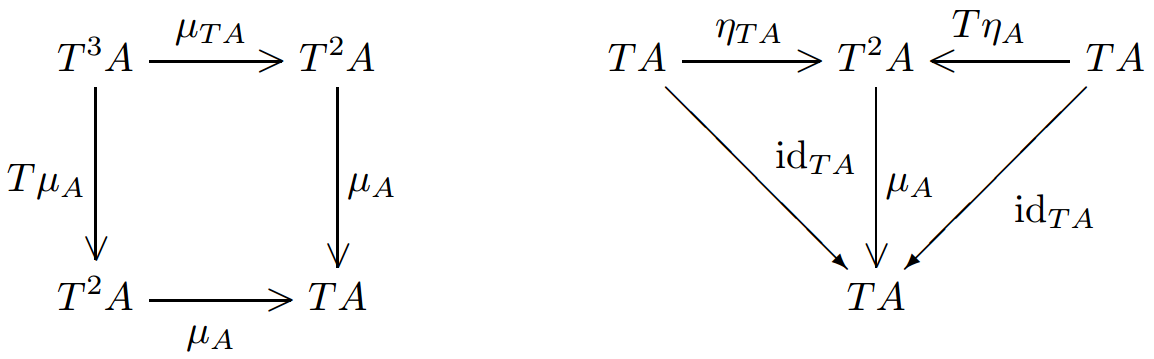
\includegraphics[width=0.7\textwidth]{monad-diagrams.png}
  \end{center}

  \vfill
  \pause

  There is a one-one correspondence between Kleisli triples and monads.
\end{frame}

\begin{frame}
  \frametitle{Monads in linguistics}

  \pause

  \begin{block}{Spot the Monad!}
    \vfill
    \begin{tabular}{rl}
      \pause $o \Rightarrow \sigma \to o$ & \\
      $\iota \Rightarrow \gamma \to \iota$ & \\
      $\bar{o} \Rightarrow \beta \to \bar{o}$ &
      \pause Reader $\delta$ ($\alpha \Rightarrow \delta \to \alpha$) \\
      \pause $\iota \Rightarrow (\iota \to o) \to o$ &
      \pause Cont $o$ ($\alpha \Rightarrow (\alpha \to o) \to o$) \\
      \pause $\iota \Rightarrow \iota \oplus *$ &
      \pause Option ($\alpha \Rightarrow \alpha \oplus *$)$$ \\
      \pause $o \Rightarrow \gamma \to (\gamma \to o) \to o$ &
      \pause StateCPS $\gamma$ $o$ ($\alpha \Rightarrow \gamma \to (\alpha \to \gamma \to o) \to o$) \\
      \pause $\bar{\iota} \Rightarrow \bar{\iota} \oplus \chi $ &
      \pause Exception $\chi$ ($\alpha \Rightarrow \alpha \oplus \chi$) \\
      \pause Ambiguities &
      \pause Set/List ($\alpha \Rightarrow [\alpha]$) \\
      \pause Probabilistic semantics &
      \pause Probability ($\alpha \Rightarrow [\mathbb{R} \times \alpha]$) \\
      \pause Hamblin alternatives &
      \pause Powerset ($\alpha \Rightarrow \alpha \to o$) \\
      \pause Potts expressives &
      \pause Writer $\epsilon$ ($\alpha \Rightarrow \alpha \times \epsilon$) \\
      \pause Rooth focus &
      \pause Pointed powerset ($\alpha \Rightarrow \alpha \times (\alpha \to o)$) \\
    \end{tabular}
  \end{block}
\end{frame}

\begin{frame}
  \frametitle{The Trouble with Monads}

  Monads observed unwieldy for multiple effects

  \vfill
  \pause

  \begin{itemize}
  \item Not easy to compose
    \begin{itemize}
    \item Monad morphisms/transformers
    \end{itemize}
  \pause
  \item Fixed stack of monad transformers
    \begin{itemize}
    \item Have to fix an order
    \end{itemize}
  \pause
  \item Fixing an order
    \begin{itemize}
    \pause
    \item Commutative?
      \begin{itemize}
      \item Order meaningless
      \item Have to manually rearrange by type conversions
      \end{itemize}
    \pause
    \item Not commutative?
      \begin{itemize}
      \item One ordering may be not expressive enough
      \item Examples of repeating transformers to express intricate interactions
      \end{itemize}
    \end{itemize}
  \pause
  \item Lifting exercises
  \end{itemize}
\end{frame}

\begin{frame}
  \frametitle{Lifting}

\begin{align*}
& \cps{\omega}{\alpha} \equiv (\alpha \to \omega) \to \omega \\
& \statecps{\gamma}{\omega}{\alpha} \equiv \gamma \to (\alpha \to \gamma \to \omega) \to \omega \\
& \exists :: (\iota \to o) \to o = \cps{o}{\iota} \\
& \dexists :: (\iota \to \statecps{\gamma}{o}{o}) \to \statecps{\gamma}{o}{o}
  = \cps{\statecps{\gamma}{o}{o}}{\iota} \\
& \dexists P \equiv \lambda e \phi. \exists (\lambda x. P x e \phi) \\
& \texttt{cont} :: \cps{\omega}{\alpha} \to \statecps{\gamma}{\omega}{\alpha} \\
& \texttt{cont}\ c \equiv \lambda e \phi. c (\lambda x. \phi x e) \\
& \texttt{fresh} :: \statecps{\gamma}{o}{\iota} \\
& \texttt{fresh} \equiv \texttt{cont}\ \exists \\
& \dexists P \equiv P \hsrevbind \texttt{fresh}
\end{align*}

\end{frame}


\begin{frame}
  \frametitle{Hiding Implementation Details of Dynamics Behind Abstract Effects}

    \begin{align*}
      \sem{it} & = \lambda \psi. \psi \hsrevbind \texttt{select}_\texttt{it} \\
      \sem{every} & = \lambda n \psi.
        \dforall x. n x \dimpl (\texttt{push}\ x \hsseq \psi x)
    \end{align*}

    instead of

    \begin{align*}
       \sem{it} & = \lambda \psi e \phi. \psi (\texttt{sel}_\texttt{it} e) e \phi \\
       \sem{every} & = \lambda n \psi.
         \dforall x. n x \dimpl (\lambda e \phi. \psi x (x \occons e) \phi)
    \end{align*}
\end{frame}

%% \begin{frame}
%%   \frametitle{Effects to the Rescue}

%%   Universal algebra in category theory
%%     \begin{itemize}
%%     \item Monads
%%       \begin{itemize}
%%       \item Originated in abstract topology
%%       \item Popularized by MacLane
%%       \item Immortalized in CS by Moggi
%%       \item Used in Haskell and semantics research
%%       \end{itemize}
%%     \item Lawvere theories
%%       \begin{itemize}
%%       \item Originated in functorial semantics of universal algebra
%%       \item Adopted by Plotkin et al. to formulate computational effects
%%       \item Recognized as a successor to monads in CS
%%       \item So far, used in Eff and Idris
%%       \end{itemize}
%%     \end{itemize}
%% \end{frame}

\begin{frame}
  \frametitle{A Short History of Effects}

  \begin{itemize}
  \item Extensible Denotational Language Specifications (1994)
    \begin{itemize}
    \item Values $\oplus$ Requests for operations
    \end{itemize}
  \pause
  \vfill
  \item The effects spring (2012-\ldots)
    \begin{itemize}
    \item Programming with Algebraic Effects and Handlers
    \item Handlers in Action
    \item Programming and Reasoning with Algebraic Effects and Dependent Types
    \item Extensible Effects -- An Alternative to Monad Transformers
    \end{itemize}
  \pause
  \vfill
  \item An alternative conception of universal algebra in category theory
    \begin{itemize}
    \item Lawvere theories vs monads
    \item Forgotten by accident, now back
    \end{itemize}
  \end{itemize}
\end{frame}

\begin{frame}[fragile]
  \frametitle{Programming with Effects}

  \begin{itemize}
  \item ``Non-compositional'' operations throw exceptions containing their
  continuations
  \item Handlers react to these exceptions by providing a specific meaning to
    the effectful operations
  \end{itemize}

  \pause

\begin{lstlisting}
type choice = effect
  operation decide : unit -> bool
end;;
let c = new choice;;

let choose_all d = handler
  | d#decide () k -> k true @ k false
  | val x -> [x];;

with choose_all c handle
  let x = (if c#decide () then 10 else 20) in
  let y = (if c#decide () then 0 else 5) in
    x - y;;
\end{lstlisting}
\end{frame}

\begin{frame}
  \frametitle{Applying Effects}

  \begin{itemize}
  \item Benefits
    \begin{itemize}
    \item Effect abstraction
    \item Effect polymorphism
    \end{itemize}
  \vfill
  \item Scope of handlers ``fits'' linguistic phenomena
    \begin{itemize}
    \item 2nd order treatment of multiple extraction
    \item Other kinds of dynamic binding
    \item Modal and nominal anaphora accessibility
    \end{itemize}
  \end{itemize}
\end{frame}

\appendix
\newcounter{finalframe}
\setcounter{finalframe}{\value{framenumber}}

\begin{frame}
  \frametitle{Related Ideas}

  \begin{block}{Intension as Computation, Extension as Value}
    \textit{``Il aime bien sa maman, son papa aussi.''}
    \begin{itemize}
    \item Intension delays anaphora
    \item If intension is $\sigma \to \alpha$, what is $\sigma$?
    \end{itemize}
    \textit{``John seeks a unicorn.''}
    \begin{itemize}
    \item Intension suppresses presuppositions
    \end{itemize}

    \vfill

    Idea:
    \begin{itemize}
    \item intension = effectful computation
    \item ambiguities = underspecified order of evaluation
    \item $\uparrow$ and $\downarrow$ = \texttt{quote} and \texttt{eval}
      (multi-stage programming?)
    \end{itemize}

    It's old:
    \begin{itemize}
    \item Making Computational Sense of Montague's Intensional Logic (JR
      Hobbs, 1978)
    \end{itemize}
  \end{block}
\end{frame}

\setcounter{framenumber}{\value{finalframe}}

\end{document}
